\section{Phân tích độ nhạy và luật quyết định}
\begin{longtable}[c]{l}
	\resizebox{\textwidth}{!}{
		\begin{tabular}{p{2.5cm}l|llll|llll|llll}
			\hline
			&&\multicolumn{4}{c|}{Best case} & \multicolumn{4}{c|}{Average case} & \multicolumn{4}{c}{Worst case} \\ \hline
			Optimization method & $\beta$ & ASR & $L_1$ & $L_2$ & $L_\infty$ & ASR & $L_1$ & $L_2$ & $L_\infty$ & ASR & $L_1$ & $L_2$ & $L_\infty$ \\ \hline
			\multirow{5}{*}{COV} & 0 & 100 & 13.93 & 1.377 & 0.379 & 100 & 22.46 & 1.972 & 0.514 & 99.8 & 32.3 & 2.639 & 0.663 \\
			& $10^{-5}$ & 100 & 13.92 & 1.377 & 0.379 & 100 & 22.66 & 1.98 & 0.508 & 99.5 & 32.33 & 2.64 & 0.663 \\
			& $10^{-4}$ & 100 & 13.91 & 1.377 & 0.379 & 100 & 23.11 & 2.013 & 0.517 & 100 & 32.32 & 2.639 & 0.664 \\
			& $10^{-3}$ & 100 & 13.8 & 1.377 & 0.381 & 100 & 22.42 & 1.977 & 0.512 & 99.9 & 32.2 & 2.639 & 0.664 \\
			& $10^{-2}$ & 100 & 12.98 & 1.38 & 0.389 & 100 & 22.27 & 2.026 & 0.53 & 99.5 & 31.41 & 2.643 & 0.673 \\ \hline
			\multirow{5}{*}{EAD (EN rule)} & 0 & 100 & 14.04 & 1.369 & 0.376 & 100 & 22.63 & 1.953 & 0.512 & 99.8 & 31.43 & 2.51 & 0.644 \\
			& $10^{-5}$ & 100 & 13.66 & 1.369 & 0.378 & 100 & 22.6 & 1.98 & 0.515 & 99.9 & 30.79 & 2.507 & 0.648 \\
			& $10^{-4}$ & 100 & 12.79 & 1.372 & 0.388 & 100 & 20.98 & 1.951 & 0.521 & 100 & 29.21 & 2.514 & 0.667 \\
			& $10^{-3}$ & 100 & 9.808 & 1.427 & 0.452 & 100 & 17.4 & 2.001 & 0.594 & 100 & 25.52 & 2.582 & 0.748 \\
			& $10^{-2}$ & 100 & 7.271 & 1.718 & 0.674 & 100 & 13.56 & 2.395 & 0.852 & 100 & 20.77 & 3.021 & 0.976 \\ \hline
	\end{tabular}} \\
	\caption[So sánh COV và EAD trên tập MNIST]{So sánh COV và EAD trong việc tìm ra công thức elastic-net trên tập MNIST. ASR là tỷ lệ tấn công thành công. Mặc dù 2 phương pháp trên đều đạt được tỷ lệ tấn công thành công như nhau, COV không hiệu quả trong việc tạo ra các mẫu đối nghịch $L_1$. Khi $\beta$ tăng lên, EAD tạo ra các mẫu đối nghịch $L_1$ ít biến dạng hơn trong khi COV thì không bị ảnh hưởng nhiều khi thay đổi $\beta$.}
	\label{tab:tab_1}
	\\
\end{longtable}

Tác giả kiểm tra sự cần thiết của việc sử dụng thuật toán 1 để giải bài toán tấn công bằng hiệu chỉnh elastic-net trong (\ref{eq:7}) bằng cách so sánh nó với thuật toán COV thuần. Trong tài liệu (Carlini and Wagner 2017b), Carlini và Wagner đã loại bỏ điều kiện ràng buộc $\mathbf{x} \in [0,1]^p$ bằng cách thay $\mathbf{x}$ bằng $\frac{\mathbf{1} + \tanh \mathbf{w}}{2}$ với $\mathbf{w} \in \mathbb{R}^p$ và $\mathbf{1} \in \mathbb{R}^p$ là vector các với các phần tử $1$. Thuật toán tối ưu mặc định ADAM (Kingma and Ba 2014) được sử dụng để giải ra nghiệm $\mathbf{w}$ và từ đó tìm được $\mathbf{x}$. Tác giả áp dụng thuật toán COV lên (\ref{eq:7}) và so sánh với EAD trên tập MNIST với các $\beta$ khác nhau trong Bảng \ref{tab:tab_1} ở trên. Mặc dù COV và EAD thu được tỷ lệ tấn công thành công tương tự nhau, người ta quan sát thấy COV không hiệu quả trong việc tạo ra các mẫu đối nghịch $L_1$. Khi tăng $\beta$, EAD tạo ra mẫu đối nghịch $L_1$ ít nhiễu hơn, trong khi các kết quả $L_1$, $L_2$, và $L_{\infty}$ của COV thì ít chịu ảnh hưởng khi thay đổi $\beta$. Khi sử dụng các hàm thư viện TensorFlow như AdaGrad, RMSProp, SGD, người ta cũng thấy nó ít ảnh hưởng bởi $\beta$ giống như trường hợp của COV. Tác giả cũng chú ý rằng COV không thể dùng phương pháp tối ưu ISTA vì thành phần hàm $\tanh$ trong hiệu chỉnh $L_1$. Sự ít ảnh hưởng của COV cho thấy nó không phù hợp cho tối ưu elastic-net, do nó không hiệu quả cho bài toán tối ưu bằng subgradient (Duchi and Singer 2009). Với EAD, tác giả quan sát thấy sự đánh đổi giữa $L_1$ với 2 độ đo nhiễu còn lại là $L_2$, và $L_{\infty}$. Điều này là do khi tăng $\beta$ làm tăng độ thưa của nhiễu và do đó tăng $L_2$, $L_{\infty}$ . Kết quả tương tự cũng được quan sát thấy với CIFAR10.
\begin{figure}[H] % places figure environment here   
    \centering % Centers Graphic
    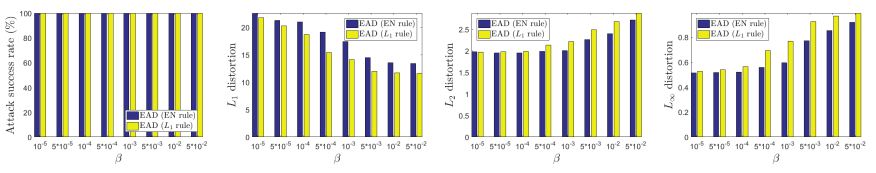
\includegraphics[width=1\textwidth]{assets/fig_02.png} 
    \caption{So sánh luật quyết định EN và $L_1$ trong EAD trên tập MNIST với nhiều tham số hiệu chỉnh $L_1$ $\beta$ (trường hợp trung bình). So sánh với luật chọn EN tại cùng giá trị $\beta$ thì luật chọn $L_1$ thu được các mẫu ít nhiễu $L_1$ hơn, nhưng đổi lại có thể bị nhiễu $L_2$, $L_{\infty}$ nhiều hơn.}% Creates caption underneath graph
    \label{fig:fg_02}
\end{figure}

Ở bảng \ref{tab:tab_1}, quá trình thuật toán tối ưu chạy để tìm ra mẫu đối nghịch cuối cùng giữa những mẫu đối nghịch thành công dựa trên hàm mất mát elastic-net trong $\{\mathbf{x}^{(k)}\}^I_{k=1}$, gọi là luật chọn elastic-net. Ngoài ra, có thể chọn mẫu đối nghịch cuối cùng sao cho $L_1$ nhỏ nhất, gọi là luật chọn $L_1$. Hình \ref{fig:fg_02} so sánh ASR và các nhiễu trung bình trên 2 luật chọn nói trên với các giá trị  khác nhau trên tập dữ liệu MNIST. Cả 2 luật chọn đều cho tỷ lệ thành công ASR $100\%$ với dải giá trị $\beta$ rộng. Với cùng 1 giá trị $\beta$, luật chọn $L_1$ cho ra các mẫu đối nghịch có nhiễu $L_1$ nhỏ hơn so với luật chọn EN, trong khi đó lại bị trả giá nhiều nhiễu hơn ở $L_2$, $L_{\infty}$. Xu hướng tương tự cũng được quan sát thấy với dữ liệu CIFAR10 (kết quả đầy đủ với cả 2 tập dữ liệu MNIST và CIFAR có trong tài liệu mở rộng). Trong các thí nghiệm tiếp theo, tác giả báo cáo kết quả của EAD với 2 luật chọn và $\beta = 10^{-3}$, vì trên tập MNIST và CIFAR10 giá trị $\beta$ làm giảm nhiễu $L_1$ trong khi có thể so sánh $L_2$, $L_{\infty}$ với trường hợp $\beta = 0$ (nghĩa là không có hiệu chỉnh $L_1$).

